\chapter{Literatuurstudie}
\label{chap:literatuurstudie}
In sectie \ref{sec:mobiele-apparaten} wordt bekeken welke mobiele apparaten er allemaal bestaan. 
Vervolgens wordt er gekeken wat er onder de motorkap van deze apparaten zit, namelijk welke mobiele besturingssystemen (\ref{sec:mobiele-besturingssystemen}), welke mobiele applicaties (\ref{sec:mobiele-applicaties}) en welke mobiele webbrowsers (\ref{sec:mobiele-webbrowsers}) er bestaan. 
Daarna komen de drie bouwblokken van het web aan bod (\ref{sec:html5-css3-js}), namelijk HTML, CSS en JavaScript.
Hierna wordt ingegaan op vele mobiele HTML5-raamwerken (\ref{sec:mobiele-html5-raamwerken}).  
Ten slotte worden verschillende, reeds bestaande manieren om raamwerken te vergelijken, bekeken (\ref{sec:vergelijken-raamwerken}).

%%%%%%%%%%%%%%%%%%%%%%%%%%%%%%%%%%%%%%%%%%%%%%%%%%%%%%%%%%%%%%%%%%
%%%%%%%%%%%%%%%%%%%%%%%%%%%%%%%%%%%%%%%%%%%%%%%%%%%%%%%%%%%%%%%%%%

\section{Mobiele apparaten}
\label{sec:mobiele-apparaten}
Mobiele apparaten bestaan in alle soorten en maten, met weinig of veel opties, voor weinig of veel geld. 
Het verdient daarom de aandacht om deze diversiteit onder de loep te nemen. 
Eerst wordt ingegaan op de soorten mobiele apparaten volgens \cite{GCF2013} en daarna op de kenmerken volgens \cite{PhilDutson2012}.

\subsection{Soorten}
Sinds de voorstelling van de Apple iPhone in 2007~\cite{David2011}, stijgt het gebruik van de smartphone ontzettend snel in onze samenleving.  
Momenteel zijn er al meer dan 1 miljard smartphones in gebruik~\cite{Yang2012}. 
Dit zal tegen 2015 verdubbeld zijn~\cite{Gillett2012}.
Foto's of video's nemen, navigeren naar het dichtstbijzijnde restaurant of nog snel het weer voor de komende dagen opzoeken, het is allemaal mogelijk. 
Hoewel Apple de lat hoog heeft gelegd met het uitbrengen van de iPhone, zijn er ook nog andere spelers op de markt. 
Zo zijn er bijvoorbeeld de op Google's Android gebaseerde smartphones zoals de Nexus 4 en de op Windows Phone gebaseerde smartphones zoals de Nokia Lumia 800.

Niet enkel de smartphone behoort tot de categorie van mobiele apparaten, maar ook de tablet. 
Tegen 2016 zulen er 760 miljoen tablets in gebruik zijn~\cite{Gillett2012}.
Ook hier kan terug gedacht worden aan één van Apple's succesvolle producten, namelijk de in 2010 uitgebrachte iPad~\cite{Apple2010}. 
Er dient echter wel opgemerkt te worden dat tien jaar voordien, Microsoft al eerder een tablet uitbracht met veel minder succes~\cite{Microsoft2000}.

De \term{e-reader} behoort tot de laatste categorie van mobiele apparaten. 
Deze wordt hoofdzakelijk gebruikt om digitale boeken te lezen, maar betere modellen laten bijvoorbeeld ook toe om te surfen op het Internet. 
Ook hier bestaat er een variëteit aan modellen zoals de Kindle van Amazon en de Reader van Sony.

\subsection{Kenmerken}
Door de vele verschillende soorten en modellen aan mobiele apparaten, is het nodig om op een hoog niveau te bekijken over welke kenmerken deze allemaal (kunnen) beschikken. 
Bij deze bespreking wordt ingegaan op de voornaamste kenmerken van smartphones en tablets. 
De kenmerken en tekst zijn gebaseerd op~\cite{PhilDutson2012}.

\subsubsection{Resolutie en PPI}
Een eerste kenmerk, waar vooral Apple met haar Retina graag mee uitpakt, is de resolutie. 
Dit is het aantal pixels getoond op het beeldscherm en wordt uitgedrukt in breedte $\times$ hoogte. 
Hoe kleiner, hoe minder er op het scherm kan worden getoond. 
Dit is vooral belangrijk wanneer veel informatie op het scherm wordt getoond. 
Bij een een kleine resolutie dient er gescrold te worden om te rest van de informatie te zien.
Een overzicht van resoluties van bekende mobiele apparaten wordt getoond op de figuur \ref{fig:resoluties}.

Indien er naast de resolutie ook nog eens rekening wordt gehouden met de fysieke grootte van het scherm, wordt er gesproken over pixels per inch~(PPI). 
De eerste iPhone had een resolutie van 320$\times$480 en een 3,5” scherm, wat neerkomt op 163 PPI. 
De iPhone4 (Retina) daarentegen heeft een resolutie van 640$\times$960 en een 3,5” scherm, wat neerkomt op 326 PPI. 
Met andere woorden zijn er meer pixels op dezelfde fysieke grootte geplaatst, wat een scherper beeld tot resultaat heeft. 

% TODO afbeelding misschien vectorieel maken:  
\begin{figure}
  \centering
  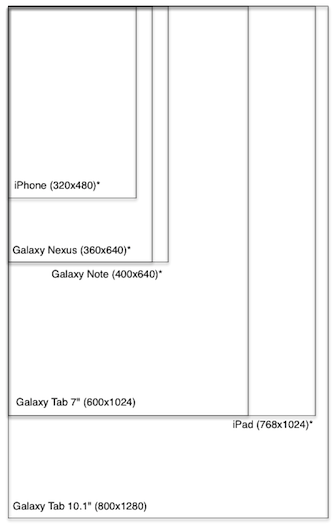
\includegraphics[height=0.8\textwidth]{figuren/mobile-devices-resolutions.png}
  \caption{Resoluties van bekende mobiele apparaten~\cite{Wolfermann2012}.}
  \label{fig:resoluties}
\end{figure}

\subsubsection{Aanraakscherm}
De populaire soorten schermen zijn resistieve en capacitieve aanraakschermen. 
De eerstgenoemde soort maakt gebruik van twee lagen die gescheiden worden door een tussenruimte. Door druk ontstaat er contact tussen de twee lagen. 
Meestal wordt bij deze soort schermen een stylus meegeleverd. 

De laatstgenoemde soort maakt gebruik van veranderingen in frequentie. 
Door het scherm aan te raken met een vinger, dat een geleider is, ontstaat er een kleine verandering in frequentie die gedetecteerd wordt. 
Niet-geleidende materialen zullen geen frequentieverandering veroorzaken, wat verklaart dat zo'n scherm niet reageert als het wordt aangeraakt met een handschoen.

\subsubsection{GPS}
Met het \term{global positioning system} (GPS) kan de gebruiker zijn locatie opvragen en doorgeven aan een applicatie om zo bijvoorbeeld het dichtstbijzijnde restaurant te vinden. 
Doordat het wat kan duren vooraleer de locatie is vastgesteld via GPS, kan het mobiel apparaat ook gebruik maken van mobiele masten of het Internet om zo, hetzij minder nauwkeurig, sneller de locatie te bepalen.

\subsubsection{Camera}
Praktisch ieder recent mobiele apparaat is uitgerust met een camera. 
Sommige bevatten zelfs twee camera's. 
De camera vooraan is veelal van mindere kwaliteit en wordt gebruikt om videogesprekken te voeren. 
Achteraan het apparaat zit dan een camera met hogere resolutie om mooie foto's te kunnen maken.

Twee andere toepassingen van de camera zijn toegevoegde realiteit en het inscannen van barcodes.
Bij het eerstgenoemde wordt informatie toegevoegd aan het beeld dat door de camera wordt geregistreerd.
Het laatstgenoemde wordt gebruikt om de populaire QR-code in te scannen en te zien wat ze betekent.
Zo'n code kan tekst bevatten, een link naar een website, een telefoonnummer, enzovoort. 

\subsubsection{Verbinding}
%TODO: Wifi, 3G, EDGE

In deze periode wil iedereen met elkaar verbonden zijn, dus ook op mobiele apparaten.
Hier wordt kort Wifi, 3G, Bluetooth en infrarood besproken.
Het mobiel apparaat kan meerdere mogelijkheden voorzien om verbinding te maken. 
Enerzijds kan dit via Wi-Fi. Daarnaast zijn er ook nog andere technologieën zoals 3G mogelijk.

% \subsubsection{Oriëntatie}
% Een handig kenmerk is dat vele mobiele apparaten kunnen detecteren hoe ze gehouden worden door de gebruiker. Dit maakt het mogelijk om de informatie zo optimaal mogelijk op het scherm te tonen. Men kan bijvoorbeeld een verschillende lay-out voorzien voor een staand en liggend scherm.
% 
% \subsubsection{Versnellingsmeter}
% Als het mobiele apparaat een versnellingsmeter bevat, is het mogelijk om hiervan in spelletjes e.d. gebruik van te maken.
% 
% \subsubsection{Afstandssensor}
% Niet veel mobiele apparaten beschikken over dit kenmerk, maar dit kan bijvoorbeeld gebruikt worden wanneer een gebruiker met zijn smartphone aan het bellen is, waarbij het scherm zichzelf automatisch uitschakelt als het tegen de wang wordt gehouden.

% \subsubsection{Fysiek toetsenbord}
% Sommige apparaten beschikken ook nog over een fysiek toetsenbord, soms ook in combinatie met een aanraakscherm. 

% \subsubsection{Barometer}
% Sommige mobiele apparaten zijn uitgerust met een barometer. Naast het meten van de druk die kan helpen bij het bepalen van het weer, helpt deze de GPS bij het bepalen van de locatie.

%TODO Sander:  Als er in de tekst naar kenmerken van een device wordt verwezen krijg je altijd het voorbeeld GPS of Camera.  Dat lijken mij ook de twee belangrijkste voor POC.  Deze twee zijn mss voldoende om dan te bespreken?

%TODO Tim: Inderdaad, of we kunnen deze kleine paragrafen allemaal in 1 grote steken.

%%%%%%%%%%%%%%%%%%%%%%%%%%%%%%%%%%%%%%%%%%%%%%%%%%%%%%%%%%%%%%%%%%
%%%%%%%%%%%%%%%%%%%%%%%%%%%%%%%%%%%%%%%%%%%%%%%%%%%%%%%%%%%%%%%%%%

\section{Mobiele besturingssystemen}
\label{sec:mobiele-besturingssystemen}
Net zoals er brede waaier bestaat aan besturingssystemen voor computers, geldt dit ook zo voor mobiele apparaten. 
In deze sectie wordt overzicht gegeven van mobiele besturingssystemen met een significant marktaandeel~\cite{David2011, Hales2012} zoals iOS en Android, maar ook een nieuwkomer op de markt, namelijk Windows Phone.
iOS en Android haalden respectievelijk 14,9\% and 75,0\% in het derde kwartaal van 2012~\cite{Protalinski2012}.

\begin{table}[t]
\centering
\begin{tabular}[b]{l r@{,}l}
\toprule
\textbf{iOS}    	& \multicolumn{2}{c}{\textbf{Marktaandeel (\%)}} \\
\midrule
6.01		& 40 & 0 \\
6.02		& 18 & 3 \\
6.1		& 17 & 5	\\
5.1.1	& 17 & 5 \\
6		& 5 & 8 \\
4.x		& 0 & 9 \\
\bottomrule
\end{tabular}
\quad
\begin{tabular}[b]{l r@{,}l}
\toprule
\textbf{Android}	& \multicolumn{2}{c}{\textbf{Marktaandeel (\%)}} \\
\midrule
2.3		& 45 & 6 \\
4.0		& 29 & 0 \\
4.1		& 12 & 2 \\
2.2		& 8 & 1 \\
2.1		& 2 & 2 \\
4.2		& 1 & 4 \\
3.0		& 1 & 3 \\
1.6 		& 0 & 2 \\
\bottomrule
\end{tabular}
\caption{Marktaandeel van iOS-versies op 14 februari 2013 en Android-versies op 4 februari 2013 \protect\cite{Sylvain2013,Android2013}.}
\label{table:marktaandeel-ios-android}
\end{table}

\subsection{iOS}
Het iPhone besturingssysteem is voor het eerst uitgekomen in juni 2007 tezamen met de iPhone. 
Later werd het hernoemd naar iPhone OS en uiteindelijk werd het iOS. 
Het is duidelijk dat iOS gebonden is aan de hardware van Apple. 
Verschillende versies volgden elkaar op: iOS 2 (juli 2008), iOS 3 (juni 2009), iOS 4 (juni 2010) en iOS 5 (oktober 2011)~\cite{Deitel2012, PhilDutson2012}. 

De nieuwste versie, iOS 6, werd uitgegeven in september 2012. 
Nieuwigheden zijn onder andere hun eigen Maps (in plaats van Google Maps) en een Pass Kit (de vervanging van het traditionele trein-, cinematicket, enz.). 
Daarnaast zijn er ook ander andere verbeteringen uitgevoerd met betrekking tot sociale media en spraakcommando's~\cite{Deitel2012}.

Op tabel \ref{table:marktaandeel-ios-android} is te zien dat bijna twee derde van de iOS-gebruikers al iOS 6 gebruikt.

Browsen op het web gebeurt met de geïnstalleerde Mobile Safari webbrowser (zie \ref{sec:mobile-safari}). Applicaties kunnen gedownload worden in de App Store, die sinds iOS 2 aanwezig is~\cite{Deitel2012}. 

\subsection{Android}
Android Inc. werd opgericht in 2003 en werd in 2005 overgekocht door Google Inc~\cite{Satyesh2012}. 
Het is net zoals iOS een mobiel besturingssysteem, maar in tegenstelling tot iOS is het open~\cite{David2011}. 
De eerste stabiele versie, Android 1.0, kwam uit in september 2008. 
Ook hier volgden verschillende versies elkaar op: Android 2.0 (oktober 2009), Android 3.0 (februari 2011) en Android 4.0 (oktober 2011)~\cite{Satyesh2012}. 
Hun nieuwste versie, Android 4.2, werd aangekondigd in oktober 2012~\cite{Sawers2012}. 

Op tabel \ref{table:marktaandeel-ios-android} is het marktaandeel te zien van de verschillende Android besturingssystemen, waargenomen over een periode van 14 dagen. 
Het is duidelijk dat Gingerbread (Android 2.3) meer dan de helft van het marktaandeel inneemt.
Applicaties worden gedownload in Google Play. 
Android bevat ook een standaard browser (zie \ref{sec:android-browser}).

\subsection{Windows Phone}
Windows Phone van Microsoft werd aangekondigd in oktober 2010 als vervanging voor Windows Mobile~\cite{Seitz2010,Lieberman2010}. 
Dit is duidelijk te zien als er gekeken wordt naar de versies: de laatste versie was Windows Mobile 6.5.3 en de eerste versie is Windows Phone 7. 
In 2011 ging Microsoft een partnerovereenkomst aan met Nokia om zo snel de markt te kunnen overwinnen~\cite{Microsoft2011}. 
De nieuwste versie, Windows Phone 8, werd aangekondigd in oktober 2012~\cite{Reed2012}. 

%%%%%%%%%%%%%%%%%%%%%%%%%%%%%%%%%%%%%%%%%%%%%%%%%%%%%%%%%%%%%%%%%%
%%%%%%%%%%%%%%%%%%%%%%%%%%%%%%%%%%%%%%%%%%%%%%%%%%%%%%%%%%%%%%%%%%

\section{Mobiele applicaties}
\label{sec:mobiele-applicaties}
%TODO Sander: eventueel eerst voorstellen,  dan een paragraafje minivergelijking..
Er zijn drie mogelijkheden om mobiele applicaties te maken~\cite{Accenture2012,Hales2012}. Eén aanpak is het maken van een webapplicatie.
Zo'n applicatie wordt geopend vanuit de webbrowser. Een andere aanpak is een \term{native} applicatie. Hierbij zal de gebruiker de applicatie installeren op zijn apparaat. Als laatste kan een mix van de vorige gemaakt worden en dat wordt een hybride applicatie genoemd.

\subsection{Webapplicaties}
In het rapport 'The (Not So) Future Web'~\cite{Phifer2011} uit juni 2011 wordt gesteld dat tegen 2015 60\% van alle mobiele bedrijfsapplicaties en 40\% van alle mobiele consumentenapplicaties, webapplicaties zullen zijn. 
Er zijn namelijk veel voordelen~\cite{Accenture2012} verbonden aan webapplicaties.

Ten eerste heeft iedereen die een webbrowser heeft op zijn mobiel apparaat, toegang tot de applicatie.  
Dit voordeel gaat niet op voor een native applicatie dat enkel voor een specifiek platform is geschreven. 

Ten tweede, aansluitend bij het bovenstaande voordeel, moet de code slechts eenmaal worden geschreven. 
Een vaak voorkomende term die dit samenvat is WORA: \term{write once, run anywhere}~\cite{Hales2012}. 
Dit is in tegenstelling tot een native applicatie die specifiek geschreven is voor bijvoorbeeld iOS, Android en Windows Phone. 
Daar dient de code driemaal te worden geschreven \'en te worden onderhouden.

Ten derde moeten webapplicaties niet worden geverifieerd vooraleer ze worden uitgebracht. 
Dit is wel zo bij native applicaties. 
Hierdoor kan in een webapplicatie een belangrijke update snel doorgevoerd worden, terwijl de native applicatie nogmaals het verificatieproces moet doorlopen.

\subsection{Native applicaties}
Een andere mogelijk is om een native applicatie te schrijven. 
Voordelen~\cite{Accenture2012} hier zijn onder meer de snelheidswinst doordat de applicatie rechtstreeks met het besturingssysteem kan werken. 
Aansluitend bij het vorige kan ook worden geargumenteerd dat het over het algemeen een native applicatie gemakkelijker de kenmerken van het mobiel apparaat, zoals de camera of GPS, aan kan spreken. 
Ten derde blijft beveiliging nog altijd een knelpunt bij webapplicaties. Een native applicatie heeft hier minder problemen. 
Als laatste kan opgemerkt worden dat het gebruik van een winkel (\term{store}) voor het aanbieden van een applicatie als voordeel kan gezien worden, afgezien van het verificatieproces. 
De applicatiewinkel zorgt namelijk voor reclame en correcte uitbetaling bij gebruik van de applicatie.

\subsection{Hybride applicaties}
Er bestaat een mix tussen de twee voorgaande soorten van mobiele applicaties, namelijk een hybride applicatie~\cite{Accenture2012}. 
Hierbij wordt de webapplicatie verpakt in een native applicatie. 
Hierdoor kunnen specifieke kenmerken van het mobiel apparaat benaderd worden die vanuit een pure webapplicatie niet konden worden benaderd.

%%%%%%%%%%%%%%%%%%%%%%%%%%%%%%%%%%%%%%%%%%%%%%%%%%%%%%%%%%%%%%%%%%
%%%%%%%%%%%%%%%%%%%%%%%%%%%%%%%%%%%%%%%%%%%%%%%%%%%%%%%%%%%%%%%%%%

\section{Mobiele webbrowsers}
\label{sec:mobiele-webbrowsers}
Sinds 2008 wordt gesproken van het mobiele web~\cite{Hales2012}. 
Vanuit mobiele webbrowsers op tablets en smartphones wordt het web meer en meer aangesproken. 
Deze mobiele webbrowsers vormen als het ware kleine besturingssystemen, waardoor de browser zelf een platform wordt~\cite{Hales2012}. 
Ze geven namelijk toegang tot allerlei kenmerken van het mobiele apparaat zoals camera en GPS. 
Denk maar aan het heel concreet voorbeeld van Google die het besturingssysteem Chrome OS maakte op basis van de Chrome webbrowser~\cite{Hales2012}.

Vanuit het standpunt om webapplicaties te maken, is het dan ook zeer belangrijk om deze evolutie op te volgen. 
Een webbrowser haalt namelijk webpagina's op die geschreven zijn in HTML en andere technologieën. 
Doordat deze technologieën evolueren (zie \ref{sec:html5-css3-js}), zullen de webbrowsers zelf ook (moeten) mee evolueren. 
Niet iedere browser zal dit op dezelfde manier doen, waardoor er verschillen zullen ontstaan waar  rekening mee moet worden gehouden. 
Het is namelijk ongewenst dat een webapplicatie enkel op Mobile Safari werkt als de ontwikkelaar een zo breed mogelijk publiek wenst te bereiken. 

In deze sectie worden enkele mobiele webbrowsers besproken. 
Eerst komen de twee meest populaire browsers aan bod, namelijk Mobile Safari en de native Android browser~\cite{Hales2012}. 
Ze zijn beide op de WebKit browser \term{engine} gebaseerd~\cite{Oeflman2011}. 
% TODO beter beschrijven browser engine
Zo een \term{engine} zorgt ervoor dat de code van de opgehaalde webpagina wordt omgezet naar de webpagina die de gebruiker te zien krijgt. 
Daarna worden Internet Explorer Mobile en Opera Mobile kort besproken. 
Het marktaandeel van de genoemde browsers wordt getoond in tabel \ref{tbl:marktaandeel-browsers}.

% TODO toevoegen data over IE mobile
\begin{table}
\centering
\begin{tabular}[b]{l r@{,}l}
\toprule
\textbf{Mobiele webbrowser} & \multicolumn{2}{c}{\textbf{Marktaandeel (\%)}} \\
\midrule
Mobile Safari		& 61 	& 02	 	\\
Android browser		& 18 	& 30 	\\
Opera Mini			& 9 		& 84 	\\
Chrome				& 2		& 02 	\\
Andere				& 8		& 82		\\
\bottomrule
\end{tabular}
\caption{Marktaandeel mobiele webbrowsers op januari 2013~\cite{NetApplications2012}.}
\label{tbl:marktaandeel-browsers}
\end{table}

\subsection{Mobile Safari}
\label{sec:mobile-safari}
Deze webbrowser van Apple zit standaard bij iOS en kan ook enkel op dit besturingssysteem worden gebruikt. 
Apple heeft veel moeite gedaan om telkens de laatste nieuwe specificaties van HTML5 in zijn webbrowsers te implementeren~\cite{Hales2012}. 
Natuurlijk zal dit ook te maken hebben met het feit dat ze geen Flash meer ondersteunen op hun iPods, iPhones en iPads~\cite{Jobs2010}.

\subsection{Android browser}
\label{sec:android-browser}
Android biedt de native Android browser aan. 
Implementatie van de HTML5-specificaties hebben wat aangesleept, maar vanaf Android 4.0 gaat dit een stuk beter~\cite{Hales2012}. 
Daarnaast is het nu ook mogelijk om de Chrome webbrowser op mobiele apparaten te installeren.

\subsection{Internet Explorer Mobile}
Net zoals bij Windows ook Internet Explorer wordt bijgegeven, geldt dit ook voor hun mobiel  besturingssysteem. 
Bij de nieuwe Windows Phone 8 zal Internet Explorer Mobile 10 worden meegeleverd. 
Deze gebruikt dezelfde \term{engine} als Internet Explorer 10. \term{WebSockets}, \term{Web Workers}, \term{Application Cache} en \term{IndexedDB} worden hierin ondersteund~\cite{Hales2012}, meer daarover in~\ref{sec:html5-css3-js}.

\subsection{Opera Mobile/Mini}
Op het moment van schrijven is Opera Mobile 12.10 de beste mobiele HTML5-browser~\cite{Sights2012}. 
Opera heeft eigenlijk twee aparte browsers, namelijk Opera Mobile en Opera Mini. 
Bij deze laatste staat de browser \term{engine} op servers van Opera, waardoor het niet het mobiel apparaat is die de webpagina verwerkt. 
De server zal, na verwerking, deze webpagina op een gecomprimeerde manier doorsturen naar de browser op het apparaat~\cite{PhilDutson2012}.

%\subsection{Mobile Firefox / Fennec}
%Mobile Firefox 16 sleept op dit moment nog net een podiumplaats in de wacht en eindigt derde, voor Mobile Safari. Mozilla staat bekend voor zijn drijvende community. 

%%%%%%%%%%%%%%%%%%%%%%%%%%%%%%%%%%%%%%%%%%%%%%%%%%%%%%%%%%%%%%%%%%
%%%%%%%%%%%%%%%%%%%%%%%%%%%%%%%%%%%%%%%%%%%%%%%%%%%%%%%%%%%%%%%%%%

\section{HTML5, CSS3 en JavaScript}
\label{sec:html5-css3-js}
De drie bouwstenen voor webontwikkeling zijn HTML5, CSS3 en JavaScript. 
HTML5 is verantwoordelijk voor de inhoud, CSS3 voor de presentatie en JavaScript voor de functionaliteit~\cite{PhilDutson2012}. 
Hieronder worden deze bouwstenen dan ook toegelicht.

\subsection{HTML5}
Zoals uitgelegd in \cite{MacDonald2011} stopte in 1998 het W3C (World Web Consortium) met het werken aan de HTML-standaard en alle energie ging uit naar zijn opvolger: XHTML 1.0, een verbeterde HTML-versie die XML-gedreven is. 
XHTML kwam in grote mate overeen met HTML, maar de syntax was veel strikter. 
In het begin kon het zijn naam waarmaken en webontwerpers helpen betere resultaten te boeken doordat ze slechte gewoontes moesten opgeven. 
Jammer genoeg bleven de beloofde voordelen uit. 
Wat veel erger was voor de nieuwe standaard, was dat geen enkele browser klaagde indien deze strikte syntax niet werd gevolgd.

In ~\cite{MacDonald2011} staat ook de reactie die hierop kwam van het W3C.  
Ze brachten een nieuwe versie uit, namelijk XHTML 2.
De manier waarop webpagina's werden geschreven veranderde doordat vele tags waren veranderd of verwijderd. 
Daarenboven sleepte deze nieuwe standaard maar aan en aan, wat ook niet in hun voordeel was. 

In plaats van te onderzoeken wat er mis was met HTML, wat XHTML probeerde te doen, werd in 2004 onderzocht wat er ontbrak. 
Opera Software, Mozilla Foundation en Apple vormden de WHATWG (Web Hypertext Application Technology Working Group). 
Ze wilden HTML niet vervangen, maar uitbreiden en die manier moest achterwaarts compatibel zijn. Na reflectie geloofde ook het W3C in deze aanpak, weliswaar op hun eigen manier.  
Zo werd HTML5 geboren, waarbij versie 5 refereert naar waar de vorige versie, HTML 4.01, gestopt was.

HTML5 is volgens ~\cite{MacDonald2011} nog altijd in ontwerp. 
Hierdoor kunnen nieuwe kenmerken op ieder momenten worden toegevoegd.  
Er is ook nog steeds onduidelijkheid waar HTML5 ons zal brengen.  
Het W3C focust op een unieke HTML5 standaard (verwacht rond 2014) terwijl WHATWG de nieuwe markup-taal ziet als levende taal waarbij voortdurend  nieuwe dingen kunnen worden toegevoegd. 
Een belangrijke opmerking hierbij is dat het laatste woord altijd bij de webbrowserfabrikant ligt, net zoals dat het geval was met de strikte syntax in XHTML. 
Als een kenmerk niet in de browser wordt ondersteund, heeft het ook geen kans op overleven.

\subsubsection{Drie basisprincipes}
Achter HTML5 zit een filosofie die in drie basisprincipes kan worden samengevat~\cite{MacDonald2011}.  
De eerste is achterwaartse comptabiliteit. De standaard mag geen veranderingen invoeren die oudere pagina's zou doen breken. 
Ten tweede moet de standaard geen nieuwe specificaties afdwingen die door de meerderheid op een andere manier worden gedaan. 
Als laatste moeten de specificaties ook een praktisch nut hebben. 
Dit betekent dat daar waar veel vraag naar is, ook het beste opweegt om in de specificaties op te nemen.

\subsubsection{Acht technologieklassen}
HTML5 kan ook bekeken worden als de volgende acht technologieklassen~\cite{W3C2012}. 
Iedere klasse wordt met enkele concrete voorbeelden aangehaald.

\begin{description}
\item [Multimedia] De nieuwe video- en audiotags maken het mogelijk om video- en geluidsfragmenten toe te voegen zonder gebruik te maken van plug-ins van derden zoals Adobe Flash en Microsoft Silverlight.

\item [Offline en opslag]  Mobiele apparaten zijn onstabiel in hun verbinding met het Internet. HTML5 voorziet het offline werken in de \term{cache}, lokale opslag (vroeger kon dit enkel via de zogenaamde cookies) en een API om bestanden te manipuleren.

\item [Performantie en integratie]  \term{Web Workers} maken het mogelijk om langdurige JavaScript taken in de achtergrond uit te voeren zodat webapplicaties dynamisch en snel blijven.

\item [Semantiek]  Een hele hoop nieuwe tags zorgen voor meer semantiek binnen webpagina's. 
Waar voorheen de webpagina bestond uit en verzameling \code{<div>}-elementen, kan nu veel concreter worden aangegeven wat er precies binnen die tags staat. 
Dit kan voor \term{search engine optimization} (SEO) een grote impact hebben. 
Daarnaast biedt dit ook mogelijkheden voor \term{e-readers} die nu beter de pagina kunnen analyseren.

\item [CSS3]  Hand in hand met HTML5 gaat CCS3 (zie \ref{ref:css3}). 
Het laat toe om webpagina's op te maken afhankelijk van het formaat van het mobiele apparaat. 
Ook kunnen webpagina's met effecten worden uitgebreid. 

\item [3D, grafieken en effecten]  De nieuwe \code{<canvas>}-tag in samenwerking met enkele lijnen JavaScript zijn enorm krachtig om eenvoudig tekeningen en animaties zelf te programmeren.

\item [Verbinding]  \term{Events} aan server zijde kunnen data naar \term{WebSockets} pushen. Hierdoor moet de webpagina niet meer voortdurend de server raadplegen, wat veel efficiënter is.

\item [Toegang tot het apparaat] Webapplicaties kunnen meer en meer kenmerken zoals camera en GPS aanspreken net zoals native applicaties dat kunnen. 
\end{description}

Er dient opgemerkt te worden dat aangehaalde klassen zoals CSS3 en geolocatie niet tot de specificaties van HTML5 behoren. 
Toch worden ze onder de koepel van HTML5 gezien~\cite{MacDonald2011}.

\subsubsection{Kenmerken detecteren en opvullen}
\paragraph{Kenmerken detecteren}
Door enerzijds de levendigheid van HTML5 en anderzijds het verdeelde landschap van browsers en besturingssystemen, worden niet alle kenmerken van HTML5 overal ondersteund. 
Een eerste mogelijkheid is om zelf op te zoeken welke kenmerken op welke apparaten werken. 
Dit kan gecontroleerd worden op bijvoorbeeld \exturl{www.caniuse.com} en \exturl{www.mobilehtml5.org}~\cite{MacDonald2011}. 

Wat nog handiger is, is om op het apparaat zelf te detecteren of het gewenste kenmerk beschikbaar is. 
Een erg handige tool hiervoor is Modernizr~\cite{Modernizr2012}. 
Het toevoegen van dit JavaScript-bestand creëert een JavaScript-object dat voor elk kenmerk teruggeeft of het al dan niet in de gebruikte browser wordt ondersteund.

\paragraph{Kenmerken opvullen}
Wanneer eenmaal gedetecteerd is dat een kenmerk niet aanwezig is, zijn er twee mogelijkheden: ofwel terugvallen op een alternatief of simuleren van dat kenmerk. 
Een voorbeeld van dit eerste kan gebeuren bij het gebruiken van de \code{<video>}-tag. 
Indien dit niet wordt ondersteund, kan worden teruggevallen op de Adobe Flash plug-in. 
Voor het simuleren van een kenmerk wordt gebruik gemaakt van \term{polyfills}. 
Dit zijn alternatieven op basis van JavaScript waarbij de native functionaliteit die normaal moet aanwezig zijn, geëmuleerd wordt~\cite{MacDonald2011,Weyl2011}.

\paragraph{Progressive enhancement en graceful degradation}
\label{par:progressive-enhancement}
Er dient een onderscheid te worden gemaakt tussen de begrippen \emph{progressive enhancement} en \emph{graceful degradation}~\cite{Hens2012}. 
Bij de eerstgenoemde wordt gestart met de basis HTML.
Deze code wordt door iedere browser op een goede manier weergegeven. 
Daarna zullen er iteratief elementen worden toegevoegd tot het moment dat de betreffende browser een bepaald kenmerk niet meer ondersteund.

De tegenhanger hiervan is \emph{graceful degradation}. 
Hierbij wordt eerst een versie ontwikkeld die enkel in de meest recentste browser kan worden getoond. 
Daarna, als de ontwikkelaar nog tijd heeft, gaat hij \term{fallbacks} implementeren waardoor minder recente browsers de applicatie ook kunnen weergeven.

\subsubsection{HTML5e}
Een bedrijf wil enerzijds een stabiele webapplicatie en wil anderzijds ook van deze nieuwe kenmerken zoveel mogelijk gebruik gaan maken. 
De term HTML5e~\cite{Hales2012} omvat de vijf meest ondersteunde HTML5-kenmerken in browsers. 
Op figuur \ref{fig:html5e} wordt een tabel getoond met de kenmerken die voor mobiele webbrowsers van toepassing zijn.

\begin{figure}
  \centering
  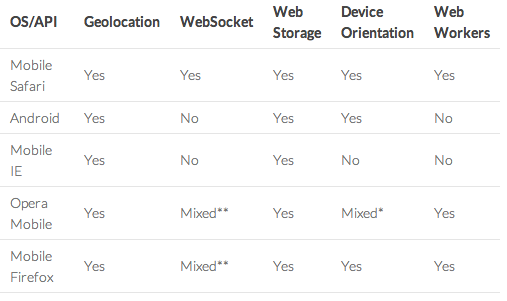
\includegraphics[width=0.8\textwidth]{figuren/html5e}
  \caption{HTML5e mobiele ondersteuning~\cite{Hales2012}}
  \label{fig:html5e}
\end{figure}

\subsection{CSS3}
\label{ref:css3}
Hand in hand met HTML5 gaat CSS3, dat zorgt voor de presentatie. 
Het is namelijk het hart van webdesign. 
CSS3 heeft hetzelfde probleem zoals HTML5 als het aankomt op de ondersteuning bij browsers~\cite{MacDonald2011}. 
Ook hier is er dus een brede waaier aan kenmerken die nog niet overal worden ondersteund. 
Kenmerken die enkel in een bepaalde browser ondersteund worden, worden voorafgaan door een browserprefix (zoals \code{-webkit-} voor WebKit gebaseerde browsers en \code{-o-} voor Opera).

In deze sectie worden kort de belangrijke eigenschappen besproken zoals \term{media queries}, effecten en lettertypes aan de hand van~\cite{MacDonald2011}.

\subsubsection{Media queries}
Zoals aangehaald, zijn er verschillende apparaten met verschillende schermen en resoluties. 
Een goeie webpagina bestaat erin deze elementen zo goed mogelijk te benutten. 
Dit kan vanaf nu door gebruik te maken van \term{media queries} in CSS3. 
De website kan zich hiermee aanpassen aan het apparaat waarop het wordt getoond. 
Dit wordt in het Engels omschreven als \term{responsive design}.
% TODO nederlands woord voor responsive design

Ook CSS3 volgt het principe van achterwaartse compatibiliteit. 
Browsers die deze \term{media queries} niet ondersteunen, zullen deze negeren en enkel de gewone lay-out toepassen ongeacht het toestel.

\subsubsection{Effecten}
Transparantie, afgeronde hoeken, schaduw en kleurenverloop zijn maar enkele van de nieuwe kenmerken in CSS3. 
Voorheen moest de webdesigner deze dingen vaak met afbeeldingen oplossen, maar nu kan dit allemaal gebeuren met CSS3. 
Daarnaast zijn er ook effecten als transformaties en transities. 
Zo is het mogelijk wanneer de cursor over een afbeelding gaat, deze ingezoomd en geroteerd kan worden. 

Dit is zeer vooruitstrevend om wille van twee zaken. 
Enerzijds is het gemakkelijker om dit in CSS-code dan in JavaScript-code. 
Anderzijds komt er ook meer en meer ondersteuning vanuit de hardware. 
Zo worden 3D transformaties in CSS3 versneld door de \term{graphics processing unit} (GPU)~\cite{Hales2012,Kool2012}.

\subsubsection{Lettertypes}
Een laatste kenmerk in CSS3 is de betere ondersteuning van lettertypes. 
Waar vroeger enkel gewerkt kon worden met veilige lettertypes voor het web, is het nu mogelijk om eigen lettertypes op te laden en te gebruiken op een website.

\subsection{JavaScript}
\label{ref:javascript}
JavaScript gaat terug tot in 1995, toen LiveScript~\cite{McFarland2011}. 
Het heeft een lange weg afgelegd tot nu en is niet altijd even ernstig genomen. 
Dit kwam omdat er niet werd ingezien wat er allemaal mee kon worden gedaan. 

Op dit moment is het maar al te duidelijk waar JavaScript in uitblinkt: het aanpassen van het \term{document object model} of kortweg DOM~\cite{PhilDutson2012}. 
Dit is een API voor HTML-documenten~\cite{Hegaret2004}. 
Hierdoor kunnen dynamische interfaces gecreëerd worden, kan op gebeurtenissen - zoals ergens op klikken - onmiddellijk gereageerd worden en is de website dan ook meer bruikbaar geworden door deze directe feedback~\cite{McFarland2011}.

% TODO referentie verschillende manieren intrepeteren
Het schrijven van JavaScript is niet gemakkelijk om twee redenen~\cite{McFarland2011}. 
Ten eerste, vergelijkbaar met HTML5 en CSS3, kunnen browsers JavaScript op verschillende manieren interpreteren. 
Gelukkig is er de laatste tijd veel gestandaardiseerd, maar toch blijven er nog verschillen. %TODO Sander: is dit niet wat vaag?  `veel gestandardiseerd'.  Concreet maken met referentie?
De ontwikkelaar dient dus tijdens het programmeren met deze verschillen rekening te houden. 
Ten tweede vergt het schrijven van simpele, veel voorkomende taken soms veel code.

Een oplossing voor de bovenstaande pijnpunten is gebruik maken van een bibliotheek. 
Een voorbeeld hiervan is de populaire jQuery Core bibliotheek. 
Het is ook mogelijk om jQuery uit te breiden met verscheidene plug-ins om de functionaliteit nog te vergroten~\cite{McFarland2011}.

%%%%%%%%%%%%%%%%%%%%%%%%%%%%%%%%%%%%%%%%%%%%%%%%%%%%%%%%%%%%%%%%%%
%%%%%%%%%%%%%%%%%%%%%%%%%%%%%%%%%%%%%%%%%%%%%%%%%%%%%%%%%%%%%%%%%%

%TODO Tim: waarom we de andere niet gekozen hebben

\section{Mobiele HTML5-raamwerken}
\label{sec:mobiele-html5-raamwerken}

In deze sectie wordt ingezoomd op bestaande mobiele HTML5-raamwerken die gebruik maken van de laatste nieuwe technologieën zoals HTML5, CSS3 en JavaScript.
Doordat deze raamwerken als paddestoelen uit de grond komen, is het onmogelijk om deze allemaal te bespreken en te vergelijken.
Hierdoor werden acht raamwerken geselecteerd waaruit uiteindelijk 4 raamwerken gedetailleerd besproken en vergeleken zullen worden in respectievelijk hoofdstukken \ref{chap:raamwerken} en \ref{chap:vergelijking}.

De raamwerken zelf worden gecategoriseerd volgens twee courante aanpakken~\cite{Oeflman2011}: opmaakgedreven en JavaScript-gedreven. 
Bij een opmaakgedreven aanpak wordt de webapplicatie voornamelijk in HTML-code geschreven. 
Daarentegen wordt bij een JavaScript-gedreven aanpak hoofdzakelijk in JavaScript geprogrammeerd.

% paragraaf per framework
% - welk framework (markup / javascript)
% - korte geschiedenis en versie
% - bedrijf, licentie

\subsection{\jqm} % TIM
\jqm{} is een opmaakgedreven raamwerk dat werd aangekondigd in 2010 en hoofdzakelijk gebruikersinterface-elementen (GI-elementen) aanbiedt~\cite{Resig2010}.
Het raamwerk wordt beheerd door het jQuery Project dat onder andere jQuery Core beheert en waar \jqm{} afhankelijk van is~\cite{JQuery2012}. 
Op het moment van schrijven zit \jqm{} aan versie~1.3.1~\cite{Parker2013b}. 
Sinds september 2012 is het enkel nog mogelijk om \jqm{} onder de Massachusetts Institute of Technology (MIT) licentie te verkrijgen~\cite{Dmethvin2012}. 
Dit betekent dat de code wordt vrijgegeven als \term{open-source} en dat deze tegelijkertijd kan worden gebruikt in propriëtaire projecten en applicaties~\cite{PhilDutson2012}.

\subsection{Sencha Touch}% SANDER
Sencha Touch wordt ontwikkeld door Sencha,  een bedrijf dat in 2010 is ontstaan als een samensmelting van Ext JS,  jQuery Touch en Raphaël.
Ext JS kan beschouwd worden als de voorganger van Sencha Touch. 
Sencha Touch is net als Ext JS een JavaScript-gedreven raamwerk met een MVC-architectuur.
Alle functionaliteit wordt dus in JavaScript-geschreven en MVC bepaalt de implementatie.
% TODO tim: is dat niet zo voor ieder raamwerk?
Het aanroepen van het raamwerk gebeurt door het invoeren van de Sencha Touch bibliotheek binnen \code{<script>}-elementen.
Sencha Touch is gratis binnen een commerciële context waarbij het bedrijf in kwestie de broncode niet deelt voor zijn gebruikers.  
Wanneer je dit wel wil doen bestaat er ook een gratis \term{open-source} versie van Sencha Touch.
Op het moment van schrijven is Sencha Touch aan versie 2.1.1~\cite{Inc.}. 

\subsection{Kendo UI} % SANDER
%TODO tim: het zijn allemaal HTML5 raamwerken, dus mss overbodig om dat als startzin van ieder raamwerk te gebruiken
Kendo UI is een HTML5-raamwerk van de hand van Telerik.
Buiten Kendo UI is Telerik voornamelijk gericht op \term{tools} voor de ontwikkelaar.
Zo ontwikkelen ze DevTools dat een grafische gebruikersinterface aan .NET ontwikkelaar aanbiedt.
Ze voorzien ook Icenium voor de ontwikkeling van hybride applicaties en kan men zien als de tegenhanger van Kendo UI dat webapplicaties aanbiedt.
Kendo UI bestaat uit drie luiken:  Web, Mobile en DataViz.  
Het eerste is gericht op de ontwikkeling van desktop en mobiele applicaties,  het tweede voegt een \term{native look-and-feel} toe aan mobiele applicaties en het laatste zorgt voor data visualisatie met HTML5- en JavaScript-technologie.
Kendo UI is een JavaScript gedreven raamwerk met een MVVM architectuur dat steunt op de jQuery bibliotheek.
Verder heeft de ontwikkelaar ook de mogelijkheid om eenvoudig de \term{backend} in integreren aan de klantzijde.
.NET,  PHP en JSP zijn momenteel de ondersteunde \term{server side wrappers}.
Een licentie voor Kendo UI waarbij één van voornoemde \term{wrappers} mogelijk is kost $\$999$.
Zonder \term{backend} integratie betaal je $\$300$ minder.
Op het moment van schrijven is Kendo UI aan versie 2013 Q1~\cite{Telerik}. 


\subsection{\lungo} % TIM
\lungo{} is een opmaakgedreven raamwerk waarbij versie~1.0 uitkwam in 2011~\cite{TapQuo2011}.
Het raamwerk wordt onderhouden door TapQuo dat een Spaans bedrijf is, gespecialiseerd rond mobiele gebruikerservaring~\cite{TapQuo2013a}.
Analoog met \jqm{} is \lungo{} afhankelijk van een JavaScript-bibliotheek, namelijk \quo{}.
\lungo{} biedt vooral GI-elementen aan, maar daarnaast zijn er ook \term{wrappers} voor cache, opslag en SQL beschikbaar~\cite{TapQuo2013}.
Net zoals \jqm{} wordt geen programmeerstijl zoals MVC afgedwongen.
Het raamwerk wordt onder de GPLv3-licentie vrijgegeven.
Een commerciële versie is mogelijk.
Op het moment van schrijven zit \lungo{} aan versie~2.1~\cite{TapQuo2013}.



\subsection{The M-Project} % SANDER

% TODO deze tekst zal later moeten worden verplaatst
%Een ander raamwerk, genaamd The-M-Project~\cite{Panacoda2012}, dwingt het Model-View-Controller (MVC) echter wel af. 
%Met dit raamwerk is het mogelijk om webapplicaties te maken die het \jqm{} raamwerk gebruiken. 
%In plaats van HTML5-code te schrijven, zoals dat bij \jqm{} gebeurt, schrijft je JavaScript-code. 
%The-M-Project zal dan zelf intern deze JavaScript-code omzetten naar de desbetreffende \jqm{} HTML5-code.

%TODO tim: referenties?
%TODO tim: schrijfwijze TPM
%TODO tim: het zijn allemaal HTML5 raamwerken, dus mss overbodig om dat als startzin van ieder raamwerk te gebruiken
The M-Project is een JavaScript/HTML5-raamwerk dat bouwt op jQuery en jQuery Mobile.
Origineel werd het in 2012 ontwikkeld door M-Way Solutions maar nu behoort het tot Panacoda,  een duitse ontwikkelaar voor software \term{tools} en mobiele web applicaties.
Panacoda bezit ook Espresso,  een krachtige \term{tool} om applicaties te bouwen en ontwikkelen met The M-Project.
Het laat ook toe applicaties om te vormen tot \term{native} applicaties. 
The M-Project is \term{open-source},  vrijgegeven onder een MIT licentie en op GitHub te vinden.
Dit raamwerk is volledig JavaScript gedreven en steunt op de MVC architectuur.
Ook ondersteunt het HTML5- en CSS3-kenmerken zoals offline  beschikbaarheid en lokale opslag.
Op het moment van schrijven is The M-Project aan versie 1.4..  
Het is belangrijk op te merken dat in de zomer van 2013 versie 2.0 wordt verwacht.  
The M-Project zal van nul worden opgebouwd omdat enkel de code aanpassen niet meer voldoende bleek.  
De voornaamste werkpunten zijn performantie en platformonafhankelijkheid~\cite{Panacoda,Laubach2013}.

\subsection{\moobile} % TIM
Een raamwerk dat nog heel jong in de schoenen staat is \moobile{}.
Op het moment van schrijven zit het raamwerk aan versie~0.2.1 sinds de eerste \term{commit} op GitHub in 2011~\cite{Dery2013}.
Het raamwerk is JavaScript-gedreven, volgt de MVC-architectuur en wordt onderhouden door de Canadees Jean-Philippe Déry.
Zelf biedt \moobile{} voornamelijk GI-elementen aan, maar deze blijven (voorlopig) beperkt tot zeven componenten en drie schermovergangen. 
Voor een gedetailleerd overzicht wordt verwezen naar~\cite{Dery2013}.
\moobile{} ontbreekt echter ondersteuning voor formulieren.
Een bijzonderheid is dat de lay-out van de componenten gemimiekt kunnen worden zodat ze de \term{look-and-feel} van een Android- of iOS-apparaat nabootsen.
Bij het raamwerk is een simulator en tool aanwezig om de volledige applicatie te maken.
Deze laatstgenoemde zorgt automatisch voor compressie van de verschillende bestanden.


\subsection{DaVinci}% SANDER 
%TODO tim: referenties?
DaVinci bestaat uit twee tools:  DaVinci Studio en DaVinci Animator.
De nadruk bij dit raamwerk ligt voornamelijk bij de generatie van code in een WYSIWYG omgeving.
De DaVinci Studio is een Eclipse plug-in die HTML-,  JavaScript- en CSS-code genereert.
De gebruiker kan UI elementen via \term{drag-and-drop} aan de applicatie toevoegen.
Het binden van data kan door op een visuele manier de mapping tussen UI en data weer te geven.
Het testen van de applicatie kan op een bijgeleverde emulator in een \term{N-screen} omgeving die de applicatie op verschillende layouts kan weergeven.
Het raamwerk gebruikt een open architectuur dat compatibel is met andere \term{open-source} raamwerken zoals jQuery, KnockOut of Backbone.
DaVinci Animator kan gebruikt worden om animaties op basis van HTML5 en CSS3 te maken in een grafische omgeving.
In SNU Research Park te Seoul worden deze \term{tools} ontwikkeld.
Op het moment van schrijven is DaVinci toe aan versie 2.0.  
Alle documentatie is momenteel nog niet vertaald van het Koreaans naar het Engels~\cite{Incross}.


\subsection{jQTouch}% TIM

%%%%%%%%%%%%%%%%%%%%%%%%%%%%%%%%%%%%%%%%%%%%%%%%%%%%%%%%%%%%%%%%%%
%%%%%%%%%%%%%%%%%%%%%%%%%%%%%%%%%%%%%%%%%%%%%%%%%%%%%%%%%%%%%%%%%%

% SANDER: bekijken aan de hand van paper
% hier alles dat we bekeken hebben, maar zonder onze eigen inbreng
\section{Vergelijken van raamwerken} 
\label{sec:vergelijken-raamwerken}
Om de verschillende mobiele HTML5-raamwerken te kunnen vergelijken hebben we een consistente manier nodig om dit te doen.  
Op deze manier worden alle raamwerken op dezelfde manier getest.

\subsection{ISO 25010}
HTML5-raamwerken zijn software en om software te vergelijken bestaat er de ISO 25010 standaard~\cite{Standard2010}.  
Hieronder vallen twee modellen:  de productkwaliteit en de kwaliteit van het product in gebruik.  
Beide modellen beschrijven de kwaliteit van software op basis van een aantal categorieën met specifieke kwaliteitseigenschappen. 
Het beoordelen van de categorieën kan gebeuren op basis van een checklist. 
 
\subsubsection{Productkwaliteit}
De acht karakteristieken die horen bij dit model zijn: functionele geschiktheid,  betrouwbaarheid,  performantie, efficiëntie, uitwisselbaarheid,  bruikbaarheid,  betrouwbaarheid, beveiligbaarheid,  onderhoudbaarheid en overdraagbaarheid.   
Vanzelfsprekend zijn niet alle categorieën even toepasbaar op HTML5-raamwerken.  
Beveiligbaarheid is bijvoorbeeld niet zo belangrijk bij mobiele HTML5-raamwerken.  
Performantie en overdraagbaarheid dan weer wel.

\subsubsection{Kwaliteit in gebruik}
De vijf karakteristieken voor dit model zijn: effectiviteit,  efficiëntie,  voldoening,  vrijheid van risico en context dekking. 
Elke karakteristiek kan toegewezen worden aan verschillende activiteiten van belanghebbenden. 
Weer zijn alle categorieën niet even toepasbaar.  
De risico die een mobiele webapplicatie meebrengt is niet van belang,  het moet vooral efficient zijn en voldoening scheppen.

De kwaliteit voor een systeem in gebruik wordt bepaald door de kwaliteit van de software,  de hardware en het besturingssysteem samen met de gebruikers, hun taken en de sociale omgeving.  
De belanghebbenden worden opgedeeld in primaire en secundaire gebruikers.  
De eerste zijn de personen die het systeem gebruiken. 
De laatste zijn diegene die zorgen voor het onderhoud.

\subsection{Bestaande use cases}
Op het web en in de literatuur kunnen we ook \term{use cases} terugvinden waar de proef op de som wordt genomen en twee of meer raamwerken met elkaar worden vergeleken.  
Deze werkwijze verschilt van \term{use case} tot \term{use case}

\subsubsection{Codefessions}
Op een blogpost van Codefessions wordt een vergelijking gemaakt tussen jQuery Mobile, Sencha Touch, jQTouch en Kendo UI~\cite{Sarrafi2012}.  
Als referentiesysteem gebruiken ze zeven criteria.  De eerste drie zijn de native \term{look-and-feel}, performantie en platform-onafhankelijke capaciteiten.  
Deze worden gequoteerd met een cijfer van 0 tot 5 waarbij 5 staat voor de maximale score. 
Kenmerken worden gequoteerd door de raamwerk met elkaar te vergelijken.  
Het raamwerk met de meeste kenmerken krijgt een 5, het tweede beste een 4, enzovoort.  
Op een analoge manier wordt code efficiëntie en gebruiksgemak gequoteerd.  
Het raamwerk dat de minste lijnen code vereist, krijgt de perfecte score. 
Hierbij moeten wel alle bestanden gerekend worden die het raamwerk nodig heeft om functioneel te zijn. 
Licenties krijgen een score van 0 tot 5 waarbij 0 betekent dat het niet beschikbaar is voor een individuele ontwikkelaar en 5 dat het raamwerk \term{open-source} en gratis te gebruiken is. 
Andere factoren zoals omkadering en uitbreidbaarheid worden niet in de vergelijkingstabel opgenomen omdat ze afhangen van de interesse van de gebruiker.  
Ze worden echter wel bekeken.

% \subsubsection{jQuery UI vs Kendo UI}
% Een andere, meer grondige vergelijking is te vinden op \exturl{www.jqueryuivskendoui.com}~\cite{Bristowe}.  Deze webpagina bestaat uit één grote tabel die meer specifieke kenmerken tussen beide raamwerkenen vergelijkt.  Er worden geen scores uitgedeeld. In de tabel vinden we onder andere een vergelijking van beschikbare thema's,  browser compatibiliteit,  form validatie,  ondersteuning van het product etc.
%TODO meer relevante use cases toevoegen

\subsection{Vergelijkingstabellen}
Naast ISO standaarden of al bestaande use cases, kunnen we ook tabellen raadplegen die zoveel mogelijk raamwerken en zoveel mogelijk kenmerken naast elkaar zetten.  
Op Wikipedia creëerde men bijvoorbeeld zo'n tabel voor JavaScript raamwerken~\cite{Wikipedia}.  

Specifiek voor mobiele HTML5-raamwerken bestaat er ook zo'n tabel,  te vinden op \exturl{www.markus-falk.com/mobile-frameworks-comparison-chart}~\cite{Falk2011}.  
We zien er een matrix met als rijen de verschillende raamwerken en in de kolommen de vergelijkingscriteria.  
Deze laatste worden opgedeeld in compatibiliteit met het besturingssysteem,  doel van de applicatie,  taal voor ontwikkeling,  hardware interactie,  UI,  licenties en andere.  
Deze laatste categorie bevat de criteria of er al-dan-niet een SDK beschikbaar is, encryptie ondersteund wordt en of advertenties worden ondersteund.  
Handig hierbij is dat de webpagina een stappenplan voorziet waarin je per categorie al je vereisten moet invullen.  
De resultaten zijn dan de raamwerken die compatibel zijn met je vereisten.

%%% Local Variables: 
%%% mode: latex
%%% TeX-master: "masterproef"
%%% End: 
